    \documentclass[10pt,aspectratio=169]{beamer}

% --- PACOTES ESSENCIAIS ---
\usepackage[utf8]{inputenc}
\usepackage[portuguese]{babel}
\usepackage{amsmath}
\usepackage{amssymb}
\usepackage{booktabs}
\usepackage{xcolor}
\usepackage{array}
\usepackage{graphicx}

% --- CONFIGURAÇÕES DE TEMA E CORES ---
\usetheme{Madrid}
\usecolortheme{whale}


\definecolor{darkblue}{RGB}{20, 40, 80}
\definecolor{midblue}{RGB}{40, 90, 150}
\definecolor{lightblue}{RGB}{242, 246, 250}
\definecolor{accentorange}{RGB}{211, 84, 0}

\setbeamercolor{palette primary}{bg=darkblue, fg=white}
\setbeamercolor{palette secondary}{bg=midblue, fg=white}
\setbeamercolor{palette tertiary}{bg=darkblue, fg=white}
\setbeamercolor{structure}{fg=darkblue}
\setbeamercolor{titlelike}{parent=palette primary}
\setbeamercolor{block title}{bg=midblue, fg=white}
\setbeamercolor{block body}{bg=lightblue, fg=black}

\setbeamerfont{title}{size=\Large, series=\bfseries}
\setbeamerfont{frametitle}{size=\large, series=\bfseries}
\setbeamertemplate{itemize items}[circle]

\setbeamertemplate{navigation symbols}{}

% --- INFORMAÇÕES DA CAPA ---
\title[Regressão Linear Bayesiana]{Regressão Linear com Enfoque Bayesiano}
\subtitle{\textit{Combined Cycle Power Plant}}
\author[Estatística Bayesiana]{Disciplina: Estatística Bayesiana}
\date{\today}

\begin{document}

% --- SLIDE 1: CAPA ---
\begin{frame}[plain]
    \titlepage
\end{frame}

% --- SLIDE 2: INTRODUÇÃO (CONTEXTO) ---
\begin{frame}{Introdução}{O Problema e o Conjunto de Dados}
    \begin{itemize}
        \item \textbf{Objetivo Principal:} Modelar a relação entre covariáveis ambientais e a produção líquida horária de energia elétrica.
        \item \textbf{Unidade de Medida da Resposta:} Megawatts (MW).
        \item \textbf{Dataset:} \textit{Combined Cycle Power Plant} (UCI Machine Learning Repository).
        \item \textbf{Características da Coleta:}
        \begin{itemize}
            \item Contém originalmente $n = 9568$ observações compiladas ao longo de 6 anos (2006--2011).
            \item Coletas realizadas sob períodos em que a usina operou em carga total.
            \item Os registros consistem em médias horárias obtidas por sensores especializados instalados na planta.
        \end{itemize}
    \end{itemize}
\end{frame}

% --- SLIDE 3: INTRODUÇÃO (VARIÁVEIS) ---
\begin{frame}{Introdução}{Estrutura e Descrição das Variáveis}
    \begin{table}
        \centering
        \caption{Preditores Ambientais e Variável Resposta}
        \small
        \begin{tabular}{lll}
            \toprule
            \textbf{Variável} & \textbf{Descrição} & \textbf{Unidade de Medida} \\
            \midrule
            \texttt{AT} & Temperatura Ambiente & °C \\
            \texttt{V}  & Vácuo de Exaustão & cm Hg \\
            \texttt{AP} & Pressão Atmosférica & mbar \\
            \texttt{RH} & Umidade Relativa do Ar & \% \\
            \midrule
            \textbf{\texttt{PE}} & \textbf{Potência Elétrica Líquida (Resposta)} & \textbf{MW} \\
            \bottomrule
        \end{tabular}
    \end{table}
\end{frame}

% --- SLIDE 4: INTRODUÇÃO (PARADIGMA BAYESIANO) ---
\begin{frame}{Introdução}{Abordagem Clássica vs. Abordagem Bayesiana}
    \begin{block}{O Paradigma Bayesiano}
        Diferente da regressão frequentista tradicional, a inferência bayesiana trata os parâmetros do modelo ($\boldsymbol{\beta}$ e $\sigma^2$) como \textbf{variáveis aleatórias}, permitindo a incorporação de conhecimento prévio por meio de distribuições \textit{a priori}.
    \end{block}
    \vspace{0.2cm}
    \begin{itemize}
        \item \textbf{Modelo Proposto:} Regressão linear gaussiana com prior conjugado \textbf{Normal--Gama Inversa} para o par de parâmetros $(\boldsymbol{\beta}, \sigma^2)$.
        \item \textbf{Principais Vantagens:} 
        \begin{itemize}
            \item Possibilita a derivação analítica direta (exata) da distribuição posterior conjunta.
            \item Fornece uma interpretação probabilística natural sobre os coeficientes de regressão e a variabilidade do erro.
        \end{itemize}
    \end{itemize}
\end{frame}

% --- SLIDE 5: TEORIA (MODELO GENERATIVO) ---
\begin{frame}{1. Conceito Teórico}{1.1 Modelo Generativo}
    Considere a formulação matricial clássica para o modelo de regressão linear:
    $$\mathbf{Y} = X\boldsymbol{\beta} + \boldsymbol{\varepsilon}$$
    Onde $\mathbf{Y} \in \mathbb{R}^{n}$, $X \in \mathbb{R}^{n \times p}$, $\boldsymbol{\beta} \in \mathbb{R}^{p}$ e o vetor de erros assume $\boldsymbol{\varepsilon} \sim \mathcal{N}_n(\mathbf{0}, \sigma^2 I_n)$.
    \vspace{0.2cm}
    
    A distribuição condicional do vetor de respostas é expressa como:
    $$\mathbf{Y} \mid \boldsymbol{\beta}, \sigma^2 \sim \mathcal{N}_n(X\boldsymbol{\beta},\, \sigma^2 I_n)$$
    
    Omitindo-se termos constantes, a função de \textbf{verossimilhança} do processo é dada por:
    $$L(\boldsymbol{\beta}, \sigma^2) \propto (\sigma^2)^{-n/2} \exp\left( -\frac{(\mathbf{Y} - X\boldsymbol{\beta})^\top(\mathbf{Y} - X\boldsymbol{\beta})}{2\sigma^2} \right)$$
\end{frame}

% --- SLIDE 6: TEORIA (ESPECIFICAÇÃO DA PRIOR) ---
\begin{frame}{1. Conceito Teórico}{1.2 Especificação da Distribuição Prior Conjugada}
    Define-se a estrutura hierárquica da prior para o par de parâmetros $(\boldsymbol{\beta}, \sigma^2)$:
    \begin{itemize}
        \item A variância residual $\sigma^2$ segue uma distribuição \textbf{Gama Inversa} ($\text{IG}$):
        $$\sigma^2 \sim \text{IG}(a_0, b_0) \implies p(\sigma^2) = \frac{b_0^{a_0}}{\Gamma(a_0)}(\sigma^2)^{-a_0-1} \exp\left(-\frac{b_0}{\sigma^2}\right)$$
        \item Condicionalmente a $\sigma^2$, o vetor de coeficientes $\boldsymbol{\beta}$ segue uma \textbf{Normal Multivariada}:
        $$\boldsymbol{\beta} \mid \sigma^2 \sim \mathcal{N}_p\left(\boldsymbol{\mu}_0,\, \sigma^2 \Lambda_0^{-1}\right)$$
    \end{itemize}
    \begin{block}{Prior Conjunta Normal--Gama Inversa (NIG)}
        A composição conjunta dos parâmetros resulta na especificação:
        $$(\boldsymbol{\beta}, \sigma^2) \sim \text{NIG}(\boldsymbol{\mu}_0, \Lambda_0, a_0, b_0)$$
        Onde $\Lambda_0 \in \mathbb{R}^{p \times p}$ é uma matriz de precisão \textit{a priori} simétrica definida positiva.
    \end{block}
\end{frame}

% --- SLIDE 7: TEORIA (TEOREMA DE BAYES) ---
\begin{frame}{1. Conceito Teórico}{1.3 Aplicação do Teorema de Bayes}
    A distribuição posterior conjunta dos parâmetros é proporcional ao produto da densidade amostral (verossimilhança) pela densidade conjunta \textit{a priori}:
    $$p(\boldsymbol{\beta}, \sigma^2 \mid \mathbf{Y}) \propto p(\mathbf{Y} \mid \boldsymbol{\beta}, \sigma^2)\, p(\boldsymbol{\beta}, \sigma^2)$$
    \vspace{0.1cm}
    Ao agrupar de forma ordenada as potências da variância $\sigma^2$ e os termos contidos na exponencial, a expressão conjunta torna-se:
    {\small
    $$p(\boldsymbol{\beta}, \sigma^2 \mid \mathbf{Y}) \propto (\sigma^2)^{-a_0 - 1 - \frac{n}{2} - \frac{p}{2}} \exp\left[ -\frac{1}{\sigma^2}\left(b_0 + \frac{1}{2}(\mathbf{Y} - X\boldsymbol{\beta})^\top(\mathbf{Y} - X\boldsymbol{\beta}) + \frac{1}{2}(\boldsymbol{\beta} - \boldsymbol{\mu}_0)^\top \Lambda_0 (\boldsymbol{\beta} - \boldsymbol{\mu}_0)\right) \right]$$}
\end{frame}

% --- SLIDE 8: TEORIA (COMPLETANDO O QUADRADO) ---
\begin{frame}{1. Conceito Teórico}{1.4 Álgebra e Fechamento de Quadrados}
    Expandindo as formas quadráticas do expoente associadas a $\boldsymbol{\beta}$, obtemos a seguinte relação linear-quadrática:
    $$\boldsymbol{\beta}^\top(X^\top X + \Lambda_0)\boldsymbol{\beta} - 2\boldsymbol{\beta}^\top(X^\top \mathbf{Y} + \Lambda_0 \boldsymbol{\mu}_0) + \mathbf{Y}^\top\mathbf{Y} + \boldsymbol{\mu}_0^\top\Lambda_0\boldsymbol{\mu}_0$$
    \vspace{0.2cm}
    Desta estrutura, isolamos os componentes definindo os novos \textbf{parâmetros posteriores}:
    $$\boxed{\Lambda_n = X^\top X + \Lambda_0} \quad \text{e} \quad \boxed{\boldsymbol{\mu}_n = \Lambda_n^{-1}(X^\top \mathbf{Y} + \Lambda_0 \boldsymbol{\mu}_0)}$$
    \vspace{0.2cm}
    Ao completar o quadrado em relação ao vetor $\boldsymbol{\beta}$, a expressão final reduz-se a:
    $$(\boldsymbol{\beta} - \boldsymbol{\mu}_n)^\top \Lambda_n (\boldsymbol{\beta} - \boldsymbol{\mu}_n) + \mathbf{Y}^\top\mathbf{Y} + \boldsymbol{\mu}_0^\top\Lambda_0\boldsymbol{\mu}_0 - \boldsymbol{\mu}_n^\top\Lambda_n\boldsymbol{\mu}_n$$
\end{frame}

% --- SLIDE 9: TEORIA (ATUALIZAÇÃO DE HIPERPARÂMETROS) ---
\begin{frame}{1. Conceito Teórico}{1.5 e 1.6 Atualização dos Hiperparâmetros Posteriores}
    A equivalência matemática garante que os parâmetros posteriores do modelo são atualizados analiticamente por meio das expressões:
    \begin{block}{Parâmetros da Distribuição Posterior}
        $$a_n = a_0 + \frac{n}{2}$$
        $$b_n = b_0 + \frac{1}{2}\left(\mathbf{Y}^\top\mathbf{Y} + \boldsymbol{\mu}_0^\top\Lambda_0\boldsymbol{\mu}_0 - \boldsymbol{\mu}_n^\top\Lambda_n\boldsymbol{\mu}_n\right)$$
    \end{block}
    \vspace{0.2cm}
    Dessa forma, conclui-se formalmente que a distribuição posterior conjunta é:
    $$(\boldsymbol{\beta}, \sigma^2 \mid \mathbf{Y}) \sim \text{NIG}(\boldsymbol{\mu}_n, \Lambda_n, a_n, b_n)$$
    Que pode ser fatorada recursivamente nas distribuições condicionais e marginais:
    $$\sigma^2 \mid \mathbf{Y} \sim \text{IG}(a_n, b_n) \quad \text{e} \quad \boldsymbol{\beta} \mid \sigma^2, \mathbf{Y} \sim \mathcal{N}_p(\boldsymbol{\mu}_n,\, \sigma^2 \Lambda_n^{-1})$$
\end{frame}

% --- SLIDE 10: TEORIA (INTERPRETAÇÃO BAYESIANA) ---
\begin{frame}{1. Conceito Teórico}{1.7 Interpretação Estatística do Modelo}
    Os parâmetros posteriores completos tornam-se:
    \begin{itemize}
        \item $\boldsymbol{\mu}_0$ e $\Lambda_0$: Representam, respectivamente, a expectativa e a precisão iniciais atribuídas aos coeficientes técnicos.
        \item $a_0$ e $b_0$: Governam o estado inicial de incerteza em relação ao ruído estocástico $\sigma^2$.
    \end{itemize}
    \begin{block}{A Média Posterior como Média Ponderada}
        $$\boldsymbol{\mu}_n = (X^\top X + \Lambda_0)^{-1}(X^\top \mathbf{Y} + \Lambda_0 \boldsymbol{\mu}_0)$$
        A equação explicita que a estimativa posterior dos coeficientes configura uma média ponderada combinando a informação proveniente dos dados amostrais ($X^\top \mathbf{Y}$) com o conhecimento estabelecido \textit{a priori} ($\Lambda_0 \boldsymbol{\mu}_0$).
    \end{block}
\end{frame}

% --- SLIDE 11: DADOS (CARREGAMENTO) ---
\begin{frame}{2. Dados}{Inspeção e Amostragem Computacional}
    \begin{itemize}
        \item \textbf{Volume Amostral Original:} $n = 9568$ linhas contendo $5$ variáveis contínuas.
        \item \textbf{Estratégia Computacional:} Com a finalidade de construir uma análise prática ágil e didática, extraiu-se uma subamostra aleatória de \textbf{300 observações}.
        \item \textbf{Reprodutibilidade:} Seleção aleatória estabilizada em ambiente de programação (R) utilizando a semente \texttt{set.seed(20260610)}.
        \item \textbf{Integridade do Banco:} Uma avaliação detalhada via código (\texttt{colSums(is.na(dados))}) acusou a presença de **zero** valores faltantes ou inconsistências nulas em todas as colunas do dataset amostrado.
    \end{itemize}
\end{frame}

% --- SLIDE 12: ANÁLISE DESCRITIVA (OBJETIVOS) ---
\begin{frame}{3. Análise Descritiva}{Objetivos do Estudo Exploratório}
    Antes de submeter as matrizes ao estimador bayesiano, a análise exploratória desempenha três papéis fundamentais no estudo:
    \begin{enumerate}
        \item \textbf{Avaliar a escala dimensional} de cada covariável do sistema, etapa indispensável para orientar a calibração adequada da matriz de hiperparâmetros de precisão \textit{a priori} ($\Lambda_0$).
        \item \textbf{Rastrear colinearidade} (associações lineares internas) entre os preditores ambientais para precaver redundâncias de variância.
        \item \textbf{Verificar preliminarmente a hipótese de linearidade} univariada cruzando individualmente cada preditor com a resposta de interesse (\texttt{PE}).
    \end{enumerate}
\end{frame}

% --- SLIDE 13: ANÁLISE DESCRITIVA (MEDIDAS RESUMO) ---
\begin{frame}{3. Análise Descritiva}{Resumo Estatístico das Variáveis (Amostra $n=300$)}
    \begin{table}
        \centering
        \caption{Medidas de Posição, Distribuição e Quartis}
        \label{tab:resumo}
        \resizebox{\textwidth}{!}{%
        \begin{tabular}{lcccccc}
            \toprule
            \textbf{Variável} & \textbf{Mínimo} & \textbf{1º Quartil} & \textbf{Mediana} & \textbf{Média} & \textbf{3º Quartil} & \textbf{Máximo} \\
            \midrule
            \texttt{AT} (°C)   & 2,34   & 12,49   & 19,09   & 19,23   & 26,02   & 32,95  \\
            \texttt{V} (cm Hg)  & 34,03  & 41,38   & 52,38   & 54,20   & 66,79   & 79,74  \\
            \texttt{AP} (mbar)  & 997,70 & 1009,20 & 1012,90 & 1013,54 & 1018,00 & 1031,70 \\
            \texttt{RH} (\%)    & 32,25  & 63,87   & 74,91   & 74,01   & 85,74   & 100,07 \\
            \textbf{\texttt{PE}} (MW) & 425,30 & 438,50  & 453,90  & 455,20  & 471,80  & 495,20 \\
            \bottomrule
        \end{tabular}%
        }
    \end{table}
\end{frame}

% --- SLIDE 14: ANÁLISE DESCRITIVA (VARIABILIDADE) ---
\begin{frame}{3. Análise Descritiva}{Análise de Dispersão e Variabilidade}
    \begin{table}
        \centering
        \caption{Variabilidade Marginal das Variáveis}
        \label{tab:dispersion}
        \small
        \begin{tabular}{lccc}
            \toprule
            \textbf{Variável} & \textbf{Média Amostral} & \textbf{Desvio-Padrão (DP)} & \textbf{Coeficiente de Variação (CV\%)} \\
            \midrule
            \texttt{AT} & 19,227  & 7,805  & 40,59\% \\
            \texttt{V}  & 54,205  & 12,891 & 23,78\% \\
            \texttt{AP} & 1013,544& 6,077  & 0,60\%  \\
            \texttt{RH} & 74,011  & 14,812 & 20,01\% \\
            \midrule
            \textbf{\texttt{PE}} & \textbf{455,202} & \textbf{17,906} & \textbf{3,93\%} \\
            \bottomrule
        \end{tabular}
    \end{table}
    \begin{itemize}
        \item \textbf{Destaque de Escala:} A pressão barométrica (\texttt{AP}) manifesta extrema estabilidade relativa ($\text{CV} = 0,60\%$), contrastando com a temperatura ambiente (\texttt{AT}), que exibe a dispersão proporcional mais acentuada ($\text{CV} = 40,59\%$).
    \end{itemize}
\end{frame}

% --- SLIDE 15: ANÁLISE DESCRITIVA (MATRIZ DE CORRELAÇÃO) ---
\begin{frame}{3. Análise Descritiva}{Matriz de Correlação Linear de Pearson}
    \begin{table}
        \centering
        \caption{Coeficientes de Correlação Inter-variáveis}
        \label{tab:correlacao}
        \small
        \begin{tabular}{lrrrrr}
            \toprule
            & \textbf{\texttt{AT}} & \textbf{\texttt{V}} & \textbf{\texttt{AP}} & \textbf{\texttt{RH}} & \textbf{\texttt{PE}} \\
            \midrule
            \textbf{\texttt{AT}} & 1,0000  & 0,8595  & -0,5830 & -0,5227 & -0,9524 \\
            \textbf{\texttt{V}}  & 0,8595  & 1,0000  & -0,5026 & -0,2846 & -0,8929 \\
            \textbf{\texttt{AP}}  & -0,5830 & -0,5026 & 1,0000  & 0,0939  & 0,5947  \\
            \textbf{\texttt{RH}}  & -0,5227 & -0,2846 & 0,0939  & 1,0000  & 0,3630  \\
            \midrule
            \textbf{\texttt{PE}}  & \textbf{-0,9524} & \textbf{-0,8929} & \textbf{0,5947} & \textbf{0,3630} & \textbf{1,0000} \\
            \bottomrule
        \end{tabular}
    \end{table}
    \begin{itemize}
        \item \textbf{Associação com a Resposta:} As covariáveis \texttt{AT} ($r = -0,9524$) e \texttt{V} ($r = -0,8929$) exibem forte acoplamento linear negativo com a potência gerada (\texttt{PE}).
        \item \textbf{Alerta de Colinearidade:} A forte correlação mútua observada entre a temperatura e o vácuo (\texttt{AT} e \texttt{V} com $r = 0,8595$) indica um expressivo compartilhamento de informação explicativa.
    \end{itemize}
\end{frame}

% --- SLIDE 16: HISTOGRAMAS (DISTRIBUIÇÕES MARGINAIS) ---
\begin{frame}{3. Análise Descritiva}{Distribuições Marginais (Histogramas)}
    \begin{columns}[c]
        \begin{column}{0.6\textwidth}
            \begin{itemize}
                \item \textbf{AT e V (Bimodais):} Apresentam comportamento com dois picos nítidos, sugerindo a existência de regimes operacionais distintos na usina.
                \item \textbf{AP (Simétrica):} Exibe distribuição aproximadamente Normal (em forma de sino), refletindo alta estabilidade barométrica.
                \item \textbf{RH (Assimétrica):} Assimetria à esquerda, indicando maior frequência de dias com umidade relativa elevada.
                \item \textbf{PE (Resposta):} Mimetiza o padrão bimodal da temperatura, concentrando a produção em dois patamares de potência.
            \end{itemize}
        \end{column}
        
        \begin{column}{0.4\textwidth}
            \begin{block}{Análise de Frequência e Densidade}
                \centering
                \includegraphics[width=0.98\linewidth]{histogramas.png}
            \end{block}
        \end{column}
    \end{columns}
\end{frame}

% --- SLIDE 17: DIAGRAMAS DE DISPERSÃO (RELAÇÃO COM PE) ---
\begin{frame}{3. Análise Descritiva}{Relação dos Preditores com a Resposta (PE)}
    \begin{columns}[c]
        \begin{column}{0.6\textwidth}
            \begin{itemize}
                \item \textbf{AT vs. PE ($r = -0,95$):} Fortíssima associação linear negativa. Configura-se como o preditor mais influente no rendimento energético.
                \item \textbf{V vs. PE ($r = -0,89$):} Relação negativa acentuada, embora exiba maior dispersão nos valores intermediários.
                \item \textbf{AP vs. PE ($r = 0,59$):} Correlação positiva moderada; elevações na pressão atmosférica tendem a aumentar a potência líquida.
                \item \textbf{RH vs. PE ($r = 0,36$):} Associação positiva fraca e comportamento ruidoso, sugerindo menor peso explicativo direto.
            \end{itemize}
        \end{column}
        
        \begin{column}{0.4\textwidth}
            \begin{block}{Comportamento Linear das Variáveis}
                \centering
                
\includegraphics[width=0.98\linewidth]{dispersao.png}
            \end{block}
        \end{column}
    \end{columns}
\end{frame}

% --- SLIDE 18: Regressão Linear  ---
\begin{frame}{4. Modelo de Regressão Linear}{4.1 Formalizando: Notação e Definições}
    Anteriormente dizemos que a formulação matricial para o modelo é:
    $$\mathbf{Y} = X\boldsymbol{\beta} + \boldsymbol{\varepsilon}$$
    Ou seja, na forma escalar (especificação 4.2):
    $$Y_i = \beta_0 + \beta_1 x_{i1} + \beta_2 x_{i2} + \beta_3 x_{i3} + \beta_4 x_{i4} + \varepsilon_i, \quad i = 1, \ldots, n$$

\begin{columns}[t]

% Coluna esquerda
\column{0.40\textwidth}

Onde $i = 1,2,\ldots,n$ é o índice da observação, com $n = 300$.
Definimos:

\begin{itemize}
\item $Y_i$: produção líquida de energia (MW)
\item $x_{i1}$: temperatura ambiente $AT_i$ (°C)
\item $x_{i2}$: vácuo de exaustão $V_i$ (cm Hg)
\item $x_{i3}$: pressão ambiente $AP_i$ (mbar)
\item $x_{i4}$: umidade relativa $RH_i$ (\%)
\end{itemize}

% Coluna direita
\column{0.55\textwidth}

Interpretação dos parâmetros:

\begin{itemize}
\item $\beta_1$: variação esperada em PE para cada aumento de 1°C em temperatura
\item $\beta_2$: ... ...  para cada aumento de 1 cm Hg no vácuo
\item $\beta_3$: ... ... para cada aumento de 1 mbar na pressão
\item $\beta_4$: ... ... para cada aumento de 1 pp na umidade relativa
\item $\varepsilon_i$: erro aleatório da $i$-ésima observação

\end{itemize}
\end{columns}
\end{frame}

% --- SLIDE 19: REGRESSÃO LINEAR (CONSTRUÇÃO DE X E Y) ---
\begin{frame}[fragile]{4. Modelo de Regressão Linear}{4.3 Construção das Matrizes $X$ e $\mathbf{Y}$}
    A partir das $n = 300$ observações amostradas, constrói-se computacionalmente o vetor resposta $\mathbf{Y} \in \mathbb{R}^{300}$ e a matriz de planejamento (\textit{design matrix}) $X \in \mathbb{R}^{300 \times 5}$, cuja primeira coluna corresponde ao intercepto.
    \begin{block}{Código (R)}
\begin{verbatim}
# Construção explícita das matrizes X e Y
Y <- as.matrix(dados$PE)
X <- cbind(1, as.matrix(dados[, c("AT","V","AP","RH")]))
colnames(X) <- c("Intercept", "AT", "V", "AP", "RH")

n <- nrow(X)   # número de observações
p <- ncol(X)   # número de parâmetros (intercepto + 4 covariáveis)
\end{verbatim}
    \end{block}
    \begin{itemize}
        \item Dimensão de $X$: $300 \times 5$.
        \item Dimensão de $\mathbf{Y}$: $300 \times 1$.
        \item $n = 300$ (observações) e $p = 5$ (parâmetros: intercepto + 4 covariáveis).
    \end{itemize}
\end{frame}

% --- SLIDE 20: ESPECIFICAÇÃO BAYESIANA (HIPERPARÂMETROS) ---
\begin{frame}{5. Especificação Bayesiana}{Escolha dos Hiperparâmetros \textit{a priori}}
    Adota-se o prior conjugado Normal--Gama Inversa, conforme apresentado na Seção 1:
    $$\sigma^2 \sim \text{IG}(a_0, b_0), \qquad \boldsymbol{\beta} \mid \sigma^2 \sim \mathcal{N}_p\left(\boldsymbol{\mu}_0,\, \sigma^2 \Lambda_0^{-1}\right)$$
    de forma que $(\boldsymbol{\beta}, \sigma^2) \sim \mathcal{NIG}(\boldsymbol{\mu}_0, \Lambda_0, a_0, b_0)$.
    \begin{block}{Hiperparâmetros Escolhidos (Prior Fraco/Não-Informativo)}
        $$\boldsymbol{\mu}_0 = \mathbf{0}_5, \qquad \Lambda_0 = 10^{-4} \cdot I_5, \qquad a_0 = b_0 = 0,01$$
    \end{block}
    \begin{itemize}
        \item Valores pequenos de $\Lambda_0$ refletem grande incerteza \textit{a priori} sobre os coeficientes $\boldsymbol{\beta}$ (prior difuso).
        \item Com $a_0 = b_0 = 0,01$, a distribuição IG \textit{a priori} da variância $\sigma^2$ também é pouco informativa.
        \item Esta escolha permite verificar a convergência da posterior bayesiana para o estimador clássico de Mínimos Quadrados Ordinários (MQO).
    \end{itemize}
\end{frame}

% --- SLIDE 21: ATUALIZAÇÃO BAYESIANA (CÓDIGO) ---
\begin{frame}[fragile]{6. Atualização Bayesiana}{Cálculo Computacional da Posterior}
    Com base nas expressões analíticas derivadas na Seção 1, calculam-se diretamente os hiperparâmetros posteriores $\Lambda_n$, $\boldsymbol{\mu}_n$, $a_n$ e $b_n$:
    \begin{block}{Código (R) -- Atualização Analítica em Forma Fechada}
\begin{verbatim}
# Precisão posterior: Lambda_n = Lambda_0 + X'X
Lambda_n <- Lambda_0 + t(X) %*% X

# Média posterior: mu_n = Lambda_n^{-1} (Lambda_0 mu_0 + X'Y)
Lambda_n_inv <- solve(Lambda_n)
mu_n <- Lambda_n_inv %*% (Lambda_0 %*% mu_0 + t(X) %*% Y)

# Hiperparâmetros da IG posterior
a_n <- a_0 + n / 2
b_n <- b_0 + 0.5 * (t(Y) %*% Y +
                     t(mu_0) %*% Lambda_0 %*% mu_0 -
                     t(mu_n) %*% Lambda_n %*% mu_n)
\end{verbatim}
    \end{block}
    Resultado: $a_n = 150,01$ e $b_n = 2850,664$.
\end{frame}

% --- SLIDE 22: ATUALIZAÇÃO BAYESIANA (RESULTADOS - MEDIA POSTERIOR) ---
\begin{frame}{6. Atualização Bayesiana}{Resultados: Média Posterior dos Coeficientes}
    \begin{table}
        \centering
        \caption{Vetor de Médias Posteriores $\boldsymbol{\mu}_n$}
        \small
        \begin{tabular}{lc}
            \toprule
            \textbf{Parâmetro} & \textbf{Estimativa Pontual} \\
            \midrule
            Intercepto ($\beta_0$) & 464,220183 \\
            AT ($\beta_1$)         & -1,928991  \\
            V ($\beta_2$)          & -0,276881  \\
            AP ($\beta_3$)         & 0,054413   \\
            RH ($\beta_4$)         & -0,163096  \\
            \bottomrule
        \end{tabular}
    \end{table}
    \begin{itemize}
        \item A média posterior $\boldsymbol{\mu}_n$ fornece a estimativa pontual de Bayes para cada coeficiente, sob perda quadrática.
        \item Sinais e magnitudes são consistentes com as correlações observadas na análise descritiva (Seção 3).
    \end{itemize}
\end{frame}

% --- SLIDE 23: ATUALIZAÇÃO BAYESIANA (VARIÂNCIA E DP) ---
\begin{frame}{6. Atualização Bayesiana}{Variância Posterior de $\sigma^2$ e Incerteza dos Coeficientes}
    A esperança posterior da variância residual é dada por:
    $$E[\sigma^2 \mid \mathbf{Y}] = \frac{b_n}{a_n - 1} = 19,1307 \implies \text{DP residual} \approx 4,3739 \text{ MW}$$
    \vspace{0.2cm}
    A matriz de covariância posterior dos coeficientes (condicional a $\sigma^2 = E[\sigma^2 \mid \mathbf{Y}]$) é:
    $$\text{Cov}(\boldsymbol{\beta} \mid \mathbf{Y}) = E[\sigma^2 \mid \mathbf{Y}] \cdot \Lambda_n^{-1}$$
    \begin{table}
        \centering
        \caption{Desvios-Padrão Posteriores Marginais dos Coeficientes}
        \small
        \begin{tabular}{lccccc}
            \toprule
            & \textbf{Intercepto} & \textbf{AT} & \textbf{V} & \textbf{AP} & \textbf{RH} \\
            \midrule
            \textbf{DP} & 55,563262 & 0,086409 & 0,041789 & 0,053779 & 0,022872 \\
            \bottomrule
        \end{tabular}
    \end{table}
\end{frame}

% --- SLIDE 24: ATUALIZAÇÃO BAYESIANA (TABELA RESUMO E IC) ---
\begin{frame}{6. Atualização Bayesiana}{Resumo da Posterior e Intervalos de Credibilidade 95\%}
    A distribuição marginal de cada coeficiente é $\beta_j \mid \mathbf{Y} \sim t_{2a_n}\left(\mu_{n,j},\, \frac{b_n}{a_n}[\Lambda_n^{-1}]_{jj}\right)$, com $2a_n$ graus de liberdade.
    \begin{table}
        \centering
        \caption{Resumo da Distribuição Posterior dos Coeficientes}
        \resizebox{\textwidth}{!}{%
        \begin{tabular}{lccccc}
            \toprule
            \textbf{Parâmetro} & \textbf{Média Posterior} & \textbf{DP Posterior} & \textbf{IC95\% (Inf.)} & \textbf{IC95\% (Sup.)} \\
            \midrule
            Intercepto ($\beta_0$) & 464,22018 & 55,56326 & 355,24216 & 573,19820 \\
            AT ($\beta_1$)         & -1,92899  & 0,08641  & -2,09847  & -1,75951  \\
            V ($\beta_2$)          & -0,27688  & 0,04179  & -0,35884  & -0,19492  \\
            AP ($\beta_3$)         & 0,05441   & 0,05378  & -0,05107  & 0,15989   \\
            RH ($\beta_4$)         & -0,16310  & 0,02287  & -0,20796  & -0,11824  \\
            \bottomrule
        \end{tabular}%
        }
    \end{table}
    \begin{itemize}
        \item \textbf{Atenção:} O IC95\% de \texttt{AP} contém o zero, sugerindo incerteza relevante sobre o sinal de seu efeito sobre \texttt{PE} nesta amostra.
    \end{itemize}
\end{frame}

% --- SLIDE 25: ATUALIZAÇÃO BAYESIANA (INTERPRETAÇÃO) ---
\begin{frame}{6. Atualização Bayesiana}{Interpretação dos Coeficientes Posteriores}
    \begin{itemize}
        \item \textbf{$\beta_1$ (AT):} coeficiente negativo -- temperaturas mais altas reduzem a eficiência das turbinas a gás, diminuindo a potência produzida.
        \item \textbf{$\beta_2$ (V):} coeficiente negativo -- maior vácuo de exaustão (pressão mais baixa no condensador) reduz a eficiência da turbina a vapor.
        \item \textbf{$\beta_3$ (AP):} coeficiente positivo -- maior pressão atmosférica favorece a densidade do ar nas turbinas a gás.
        \item \textbf{$\beta_4$ (RH):} coeficiente ligeiramente negativo -- umidade mais alta pode reduzir levemente o desempenho.
    \end{itemize}
\end{frame}

% --- SLIDE 26: COMPARAÇÃO COM MQO ---
\begin{frame}{7. Comparação com MQO}{Bayesiano (Prior Fraco) vs. Mínimos Quadrados Ordinários}
    Com prior não-informativo ($\Lambda_0 \to 0$), espera-se que a média posterior $\boldsymbol{\mu}_n$ convirja para o estimador clássico $\hat{\boldsymbol{\beta}} = (X^\top X)^{-1} X^\top \mathbf{Y}$.
    \begin{table}
        \centering
        \caption{Comparação: MQO vs. Bayesiano (Prior Fraco)}
        \small
        \begin{tabular}{lcc}
            \toprule
            \textbf{Parâmetro} & \textbf{MQO} & \textbf{Bayesiano} \\
            \midrule
            Intercepto & 471,834587 & 464,220183 \\
            AT         & -1,934442  & -1,928991  \\
            V          & -0,276200  & -0,276881  \\
            AP         & 0,047048   & 0,054413   \\
            RH         & -0,164198  & -0,163096  \\
            \bottomrule
        \end{tabular}
    \end{table}
    \begin{itemize}
        \item As estimativas bayesianas são praticamente idênticas às do MQO, como esperado sob prior difuso.
        \item \textbf{Diferença fundamental:} na abordagem bayesiana, $\boldsymbol{\mu}_n$ é a média de uma distribuição de probabilidade sobre $\boldsymbol{\beta}$, e os intervalos de credibilidade possuem interpretação probabilística direta -- diferentemente dos intervalos de confiança frequentistas.
    \end{itemize}
\end{frame}

% --- SLIDE 27: ANÁLISE DE RESÍDUOS (MÉTRICAS) ---
\begin{frame}{8. Análise de Resíduos}{Adequação do Ajuste}
    Utilizando os valores ajustados $\hat{\mathbf{Y}} = X\boldsymbol{\mu}_n$ e os resíduos $\mathbf{e} = \mathbf{Y} - \hat{\mathbf{Y}}$, obtêm-se as seguintes métricas de qualidade de ajuste:
    \begin{block}{Métricas de Qualidade do Ajuste}
        \begin{itemize}
            \item $R^2 = 0,94075$ -- aproximadamente $94\%$ da variabilidade de \texttt{PE} é explicada pelo modelo.
            \item $\text{RMSE} = 4,3512$ MW.
            \item $\text{MAE} = 3,5926$ MW.
        \end{itemize}
    \end{block}
    \vspace{0.2cm}
    Em seguida, investigam-se graficamente os resíduos para verificar normalidade, homocedasticidade e ausência de padrões sistemáticos.
\end{frame}

% --- SLIDE 28: ANÁLISE DE RESÍDUOS (GRÁFICOS DE DIAGNÓSTICO) ---
\begin{frame}{8. Análise de Resíduos}{Gráficos de Diagnóstico}
    \begin{columns}[c]
        \begin{column}{0.55\textwidth}
            \begin{itemize}
                \item \textbf{Resíduos vs. Ajustados:} dispersão sem padrão sistemático aparente em torno de zero, indicando homocedasticidade razoável.
                \item \textbf{QQ-plot:} pontos próximos da reta de referência, sugerindo aproximação adequada à normalidade nos resíduos.
                \item \textbf{Histograma:} forma aproximadamente simétrica e unimodal, compatível com a suposição gaussiana do modelo.
                \item \textbf{Resíduos por Ordem:} ausência de tendência ou autocorrelação visível ao longo do índice das observações.
            \end{itemize}
        \end{column}
        \begin{column}{0.45\textwidth}
            \begin{block}{Diagnóstico Gráfico dos Resíduos}
                \centering
                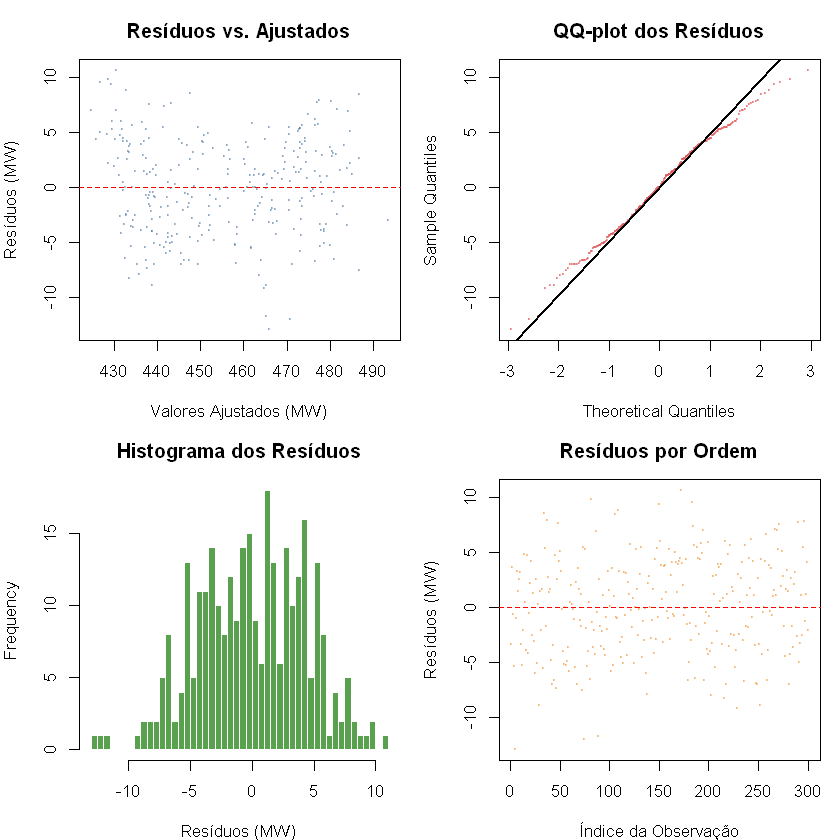
\includegraphics[width=0.98\linewidth]{residuos_diag.png}
            \end{block}
        \end{column}
    \end{columns}
\end{frame}

% --- SLIDE 29: DISTRIBUIÇÕES POSTERIORES MARGINAIS (TEORIA) ---
\begin{frame}{9. Distribuições Posteriores Marginais}{Distribuição $t$-Student dos Coeficientes}
    A distribuição marginal de cada coeficiente $\beta_j \mid \mathbf{Y}$ segue uma distribuição $t$-Student com $2a_n$ graus de liberdade:
    $$\beta_j \mid \mathbf{Y} \sim t_{2a_n}\!\left(\mu_{n,j},\; \frac{b_n}{a_n}\left[\Lambda_n^{-1}\right]_{jj}\right)$$
    \begin{itemize}
        \item Como $n = 9568$ (tamanho original do conjunto) é muito grande, e $a_n = 150,01$ também é grande, essa distribuição $t$ é essencialmente aproximada por uma Normal.
        \item As regiões sombreadas nos gráficos a seguir representam os \textbf{intervalos de credibilidade de 95\%}.
        \item A linha tracejada vertical indica a média posterior $\mu_{n,j}$ de cada coeficiente.
    \end{itemize}
\end{frame}

% --- SLIDE 30: DISTRIBUIÇÕES POSTERIORES MARGINAIS (GRÁFICO) ---
\begin{frame}{9. Distribuições Posteriores Marginais}{Densidades Posteriores dos Coeficientes}
    \begin{columns}[c]
        \begin{column}{1.0\textwidth}
            \begin{block}{Densidades Marginais $\beta_j \mid \mathbf{Y}$ com IC95\% Sombreado}
                \centering
                \includegraphics[height=6.3cm]{posteriores_marginais.png}
            \end{block}
        \end{column}
    \end{columns}
\end{frame}

% --- SLIDE 31: PREDIÇÃO (TEORIA) ---
\begin{frame}{10. Predição}{Distribuição Preditiva Posterior}
    Para uma nova observação $\mathbf{x}_\star$, a \textbf{distribuição preditiva posterior} marginaliza sobre $\boldsymbol{\beta}$ e $\sigma^2$, resultando em:
    $$Y_\star \mid \mathbf{Y} \sim t_{2a_n}\!\left(\mathbf{x}_\star^\top \boldsymbol{\mu}_n,\; \frac{b_n}{a_n}\left(1 + \mathbf{x}_\star^\top \Lambda_n^{-1} \mathbf{x}_\star\right)\right)$$
    \begin{itemize}
        \item A média da preditiva é a predição pontual $\mathbf{x}_\star^\top \boldsymbol{\mu}_n$.
        \item A escala da preditiva incorpora \textbf{duas fontes de incerteza}: a incerteza residual ($b_n/a_n$) e a incerteza sobre os próprios coeficientes $\boldsymbol{\beta}$ (termo $\mathbf{x}_\star^\top \Lambda_n^{-1} \mathbf{x}_\star$).
        \item O resultado é, novamente, uma distribuição $t$-Student com $2a_n$ graus de liberdade.
    \end{itemize}
\end{frame}

% --- SLIDE 32: PREDIÇÃO (EXEMPLO NUMÉRICO) ---
\begin{frame}[fragile]{10. Predição}{Exemplo de Predição para Nova Observação}
    Considere uma nova observação com covariáveis $AT = 20$, $V = 55$, $AP = 1010$, $RH = 70$.
    \begin{block}{Código (R) -- Função de Predição Bayesiana}
\begin{verbatim}
predicao_bayesiana <- function(x_new, mu_n, Lambda_n_inv, a_n, b_n,
                                nivel = 0.95) {
  x_star <- matrix(c(1, x_new), ncol = 1)
  media_pred  <- as.numeric(t(x_star) %*% mu_n)
  escala_pred <- sqrt(as.numeric(b_n / a_n *
                       (1 + t(x_star) %*% Lambda_n_inv %*% x_star)))
  gl_pred <- 2 * a_n
  ic_l <- media_pred - qt(0.975, df = gl_pred) * escala_pred
  ic_h <- media_pred + qt(0.975, df = gl_pred) * escala_pred
  list(media = media_pred, IC_low = ic_l, IC_high = ic_h)
}
\end{verbatim}
    \end{block}
    \begin{itemize}
        \item \textbf{Predição (média):} $451,772$ MW
        \item \textbf{IC 95\% de credibilidade:} $[443,131 \,;\, 460,413]$ MW
    \end{itemize}
\end{frame}

% --- SLIDE 33: PREDIÇÃO (AVALIAÇÃO GRÁFICA) ---
\begin{frame}{10. Predição}{Avaliação Preditiva: Observado vs. Predito}
    \begin{columns}[c]
        \begin{column}{0.55\textwidth}
            \begin{itemize}
                \item Comparação entre os valores observados de \texttt{PE} e os valores preditos $\hat{Y} = X\boldsymbol{\mu}_n$ para as primeiras 200 observações.
                \item A linha vermelha tracejada representa a reta identidade $y = x$ (predição perfeita).
                \item Os pontos concentram-se próximos a essa reta, refletindo o alto $R^2 = 0,94075$ obtido na Seção 8.
                \item Pequenos desvios são esperados e consistentes com o erro residual estimado ($\text{DP} \approx 4,37$ MW).
            \end{itemize}
        \end{column}
        \begin{column}{0.45\textwidth}
            \begin{block}{Observado vs. Predito (200 obs.)}
                \centering
                \includegraphics[width=0.98\linewidth]{obs_vs_pred.png}
            \end{block}
        \end{column}
    \end{columns}
\end{frame}

% --- SLIDE 34: SUMÁRIO FINAL ---
\begin{frame}{11. Sumário Final}{Síntese do Trabalho}
    Este trabalho implementou, passo a passo, a \textbf{regressão linear bayesiana com prior conjugado Normal--Gama Inversa} aplicada ao dataset \textit{Combined Cycle Power Plant}.
    \begin{table}
        \centering
        \small
        \begin{tabular}{ll}
            \toprule
            \textbf{Etapa} & \textbf{O que foi feito} \\
            \midrule
            Seção 2 & Carregamento e inspeção dos dados (9568 obs., 5 variáveis) \\
            Seção 3 & Análise descritiva, correlações e diagramas de dispersão \\
            Seções 4--5 & Construção das matrizes $X$, $\mathbf{Y}$ e escolha dos hiperparâmetros \\
            Seção 6 & Atualização analítica: $\Lambda_n$, $\boldsymbol{\mu}_n$, $a_n$, $b_n$ \\
            Seção 7 & Verificação: posterior $\approx$ MQO sob prior fraco \\
            Seção 8 & Diagnóstico de resíduos (normalidade, homocedasticidade) \\
            Seção 9 & Densidades marginais posteriores e IC95\% \\
            Seção 10 & Distribuição preditiva posterior e avaliação preditiva \\
            \bottomrule
        \end{tabular}
    \end{table}
\end{frame}

% --- SLIDE 35: SUMÁRIO FINAL (CONSIDERAÇÕES SOBRE O PRIOR) ---
\begin{frame}{11. Sumário Final}{Considerações sobre a Escolha do Prior}
    \begin{block}{Sobre a Escolha do Prior}
        Com $\Lambda_0 = 10^{-4} I$ e $a_0 = b_0 = 0,01$, o prior é praticamente não-informativo, e os resultados bayesianos coincidem com os do MQO clássico.
    \end{block}
    \vspace{0.3cm}
    \begin{itemize}
        \item O diferencial do arcabouço bayesiano está na \textbf{interpretação probabilística completa}.
        \item Os intervalos de credibilidade têm significado probabilístico direto sobre os parâmetros.
        \item A distribuição preditiva propaga naturalmente toda a incerteza dos parâmetros ($\boldsymbol{\beta}$ e $\sigma^2$) para a predição de novas observações.
    \end{itemize}
    \vspace{0.5cm}
    \begin{center}
        \Large \textbf{Obrigado!}
    \end{center}
\end{frame}

\end{document}